\section{Related Work and Preliminaries}
\label{sec:background-scale}



% Our method brings together the field of generalizable novel view synthesis and the study of scaling laws, common in large language models and 2D computer vision.
%
\paragraph{Generalizable novel view synthesis.} 
%
In generalizable novel view synthesis, we are given a set of $V_C$ context images paired with known camera poses and intrinsics $\ctxt = \left\{(I_i, \, \pose_i, \, \K_i) \mid i = 1, \, \ldots, \,V_C\right\}$. The typical objective is to synthesize an \emph{unseen} view of the same scene given a target camera configuration $\tpose, \tK$:
%
\begin{equation}\label{eq:view_synthesis}
\tilde{I}_T = \mathrm{Render}\big[\ctxt,  \tpose,  \tK \big].
\end{equation}

One line of work attempts to solve this problem with neural network architectures that explicitly model aspects of 3D image formation, for instance, via differentiable rendering or using epipolar line constraints~\cite{yu2020pixelnerf,sitzmann2019srns,charatan2024pixelsplat,szymanowicz2024splatter,suhail2022generalizable}. 
%
In contrast, \emph{geometry-free} methods avoid explicit geometric modeling in favor of flexibility and generality~\cite{eslami2018neural,sitzmann2021lfns,sajjadi2022scene,rombach2021geometry, sajjadi2023rust}. Here, we are primarily interested in a recently proposed subclass of these models which achieve state-of-the-art results with pure transformer architectures~\cite{jin2024lvsm, jiang2025rayzer, sajjadi2022scene, mitchel2025true}. In particular, we seek to study the ``Large View Synthesis Model'' (LVSM)~\cite{jin2024lvsm}, which achieves state-of-the-art NVS performance and serves as the prototypical instance of the view synthesis transformer. 
%in the supervised setting
% LVSM is trained with the following training loss:
% \begin{equation}
%     \mathcal{L}(I,\hat{I}) = \mathrm{MSE}(I,\hat{I}) + 0.5 \times \mathrm{LPIPS}(I,\hat{I}).
% \end{equation}
% We use the same loss for all our experiments in this paper.
LVSM can be implemented in two ways: as either an encoder-decoder model or decoder-only model. The authors' proposed decoder-only variant is far more performant, so we primarily consider this architecture (pictured in \figref{fig:lvsm-svsm}, left) in our analysis.% and comparisons. 

\begin{figure*}[t]
    \centering
    \vspace{-0.8cm}
    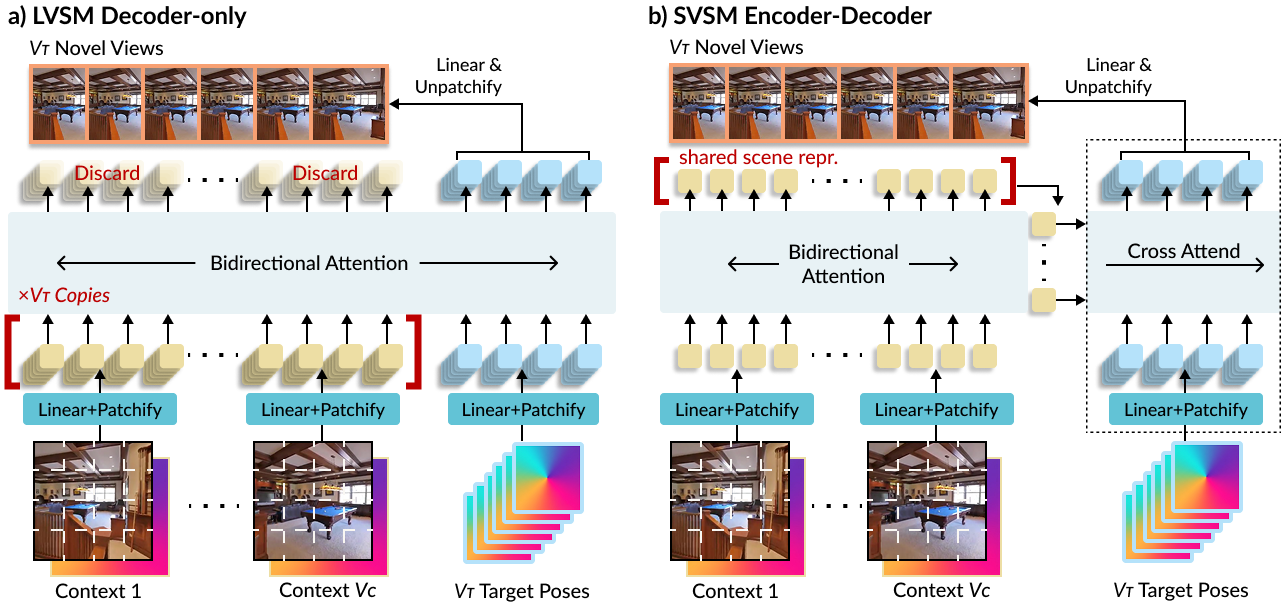
\includegraphics[width=0.9\textwidth]{images/lvsm_svsm.png}
    \caption{
        \textbf{Architectures of the current SOTA, the decoder-only LVSM~\citep{jin2024lvsm} (a) and SVSM (ours, b).} Our cross-attention based decoder enables parallel rendering of multiple target views after a single scene encoding. Each target view is decoded independently given the shared scene representation, but the cross-attention allows these independent decodings to be executed in parallel.
        \vspace{-1\baselineskip}
    }
    \label{fig:lvsm-svsm}
\end{figure*}
Decoder-only LVSM consists of a single module: A decoder $\mathcal D $ which ingests the raw context $\mathfrak C$ along with a \emph{single} target configuration, and aims to render a prediction of the target view $\tilde{I}_T =  \mathcal D \big[\mathfrak C, \tpose, \tK\big]$. This model is \emph{bidirectional} as the context view tokens are updated with information about target pose and tokens in each layer. Thus, the processed context tokens cannot be reused and must be re-initialized and updated each time a new target view is rendered. As a consequence, rendering $V_T$ target views requires $V_T$ forward passes through the full network. 
% Thus, the FLOPS on a forward pass are roughly proportional to rendering $V_T$ views of a scene with $V_C$ context views consumes
%
Decoder-only LVSM consists of standard ViT layers~\citep{dosovitskiy2020image} which apply self-attention ($\mathtt{Attn}$) followed by an MLP ($\mathtt{MLP}$). 
Therefore, the FLOPs on a forward pass scale linearly with the number of target views $V_T$
\begin{equation}\label{eqn:lvsm-flops}
\begin{split}
    \computeMLP^{\text{(LVSM)}} & \propto V_T\times (V_C+1)
    \\
    \computeAttn^{\text{(LVSM)}} & \propto V_T\times (V_C+1)^2
\end{split}
\end{equation}
where $\computeMLP^{\text{(LVSM)}}$ and $\computeAttn^{\text{(LVSM)}}$ are the FLOPs consumed by the MLP and attention in the decoder-only LVSM. In our studies, $\computeMLP^{\text{(LVSM)}}$ is the dominating factor (for more details, see \suppref{supp:flop-calcs}). In what follows, we will continue to use $\chi$ to denote the compute metric, typically measured in FLOPs.

\newpage

\paragraph{Scaling Laws.}
%
As the scale of deep learning models continues to increase, it has become increasingly important to understand the relationship between performance and compute to ensure an efficient use of resources. To this end, scaling analyses have been conducted for language models~\citep{hoffmann2022training, kaplan2020scaling}, vision transformers~\citep{zhai2022scaling}, and diffusion transformers~\citep{esser2024scaling, peebles2023scalable}. The general approach is straightforward:  train models at different compute budgets and analyze performance as a function of compute. 

Scaling studies are useful in two ways. First, they provide a predictable trend of performance with compute, essentially describing a performance metric $P$ as function of compute \compute{} which can reveal characteristic scaling behavior. For example, in language models, $P(\compute{})$ has been found to approximately follow a power-law~\citep{kaplan2020scaling}. Second, they have revealed which hyperparameter choices are most effective as models scale. For instance,  Chinchilla scaling laws~\cite{hoffmann2022training} reveal the best way to trade-off between model size $N$, measured in parameter count, and the number of training samples used, $D$. Analysis is performed by sweeping across a wide range of $N$ and $D$ to discover for compute budget $\compute{}$ the optimal $N$ and $D$. Then, taking this paired data and assuming a power law relation between $N_{\text{opt}}$ and $D_{\text{opt}}$ and $\compute{}$, one can fit powers $a$ and $b$ of $\compute{}$ to the pairings
\begin{equation}\label{eqn:chinchilla}
    N_{\text{opt}}(\compute{}) \propto \compute{}^a, D_{\text{opt}}(\compute) \propto \compute{}^b.
\end{equation}
Remarkably, experiments demonstrate $a \approx b$, suggesting  $N$ and $D$ should scale proportionally. In our study, we will focus on the second of these two kinds of studies: replicating the Chinchilla study (\secref{sec:scaling-two-view}) in the NVS domain and exploring other similar tradeoffs, such as the effective batch size (\secref{sec:effective-batch})


\paragraph{Extremely long context view synthesis.}
%
Recently, there has been a line of work aiming to develop view-synthesis and 3D-reconstruction models whose computational cost scales linearly with the number of context images~\citep{zhang2025test,wang2025continuous, ziwen2025llrm}. Indeed, as in \eqref{eqn:lvsm-flops}, as $V_C$ grows, the quadratic cost of attention comes to dominate the compute and becomes infeasible. In that regime, such linear-cost models are promising alternatives. However, we restrict our focus to sparse to moderately sparse view synthesis, for which linear-cost models are currently not state of the art.

% discovering which choices are important for scalable view synthesis models.

% (1) by predicting trends of performance with compute, they give confidence that there are benefits left to squeeze out with more scale and (2) as \textit{compute} is typically the limiting factor, knowing the best training settings for a given compute-budget is beneficial for squeezing out the most performance. 






% \begin{itemize}
%     \item Kaplan, Chinchilla, etc.
%     \item Discuss data / model size for compute optimal frontier
%     \item 
% \end{itemize}

% \lipsum[1-1]


